\documentclass[12pt]{extreport}

% Мова
\usepackage[utf8]{inputenc} % правильне кодування
\usepackage[T2A]{fontenc}
\usepackage[main=ukrainian,english]{babel}

% Розмір паперу та поля
\usepackage[a4paper,top=2cm,bottom=2cm,left=3cm,right=3cm,marginparwidth=1.75cm]{geometry}

% Корисні пакети
\usepackage{blindtext,graphicx}
\usepackage{multirow}
\usepackage[absolute]{textpos}
\setlength{\TPHorizModule}{1cm}
\setlength{\TPVertModule}{1cm}
\usepackage{amsmath}
\usepackage{graphicx}
\usepackage[colorlinks=true, allcolors=blue]{hyperref}

\title{\textbf{ЗВІТ}\\[0.5ex]\Large до лабораторної роботи \\на тему:\\\huge «Тема лабораторної роботи»}
\author{}
\date{}

\begin{document}

\begin{textblock}{10}(5.25,1.5)
\begin{center}
\noindent\Large Київський націонльний університет імені Тараса Шевченка
\end{center}
\end{textblock}

\begin{textblock}{13}(5.25,19.7)
\begin{flushright}
\noindent\Large
Виконав\\[1ex]
студент першого курсу\\
групи К-XX\\
факультету комп'ютерних\\наук та кібернетики\\[1ex]
Прізвище Ім'я
\end{flushright}
\end{textblock}

\begin{textblock}{10}(5.25,26.7)
\begin{center}
\noindent\Large
Київ, 20ХХ
\end{center}
\end{textblock}

\maketitle

\large % задає збільшений розмір шрифту для всього документу

\section*{Мета}
Звичайний текст, \textit{курсив}, \textbf{жирний}. Також \href{https://github.com/vladyslavpavlenko}{посилання}.

\section*{Основні принципи виконання роботи}
Ваш текст.\\

\noindent % прибрати відступ
Ваш текст у новому абзаці.

\section*{Виконання}
\subsection*{Підпункт}
Ваш текст.

\begin{table}[h]
\large
\centering
\begin{tabular}{|c|c|c|c|c|}
\hline
$X$ & 0 & 1 & 0 & 1\\
\hline
$Y$ & 0 & 0 & 1 & 1\\
\hline
$X\oplus Y$ & 0 & 1 & 1 & 0\\
\hline
\end{tabular}
\caption{\label{tab:widgets}Таблиця істинності операції додавання за модулем два.}
\end{table}

\begin{figure}[h]
\centering
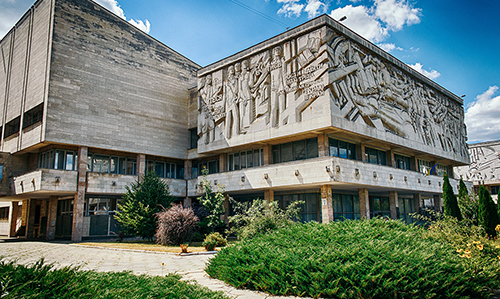
\includegraphics[width=0.7\textwidth]{fcsc.jpg}
\caption{\label{fig:fcsc}Факультет комп'ютерних наук та кібернетики.}
\end{figure}

\subsection*{Підпункт}
Ваш текст

\section*{Висновок}
Ваш висновок.

\pagebreak
\pagenumbering{gobble}
\section*{Додаток}
Ваш додаток.

\end{document}